%As mentioned in the Introduction, the main challenge of our project is to convert the mesh based geometry, obtained on a previous step, back to CAD representation. 
Parametrised geometries are often given in terms of Non-Uniform B--Spline (NURBS) descriptions (see, for example, documentation of FreeCAD software \cite{FreeCAD}). 
To define NURBS from a mathematical standpoint, we first define so-called \textit{Bezier curves} \cite{farin2002handbook} which we will use later for the definition of NURBS.
\subsection{Bezier Curves}
\emph{Bezier curve} is a \textit{parametric} curve, which is often used for producing a smooth approximation of a given set of data points.
 
An analytical expression for the Bezier curve is given by:
\begin{equation*}
\vec{B}(t)=\sum\limits_{i=0}^n b_i^n(t) \vec{P}_i
\end{equation*}
where $\vec{P}_i$ is the $i$--th control point (we have $n+1$ control points). And
\begin{equation*}
b_i^n(t)=\left(\begin{array}{c}n\\i\end{array}\right)(1-t)^{(n-i)}t^i
\end{equation*}
is the $i$--the Bernstein polynomial (see \cite{lorentz2012bernstein}) of degree $n$.

Additionally to the expression with the Bernstein polynomials, one can use a recursion formula (so-called \textbf{de Casteljau Algorithm} \cite{farin2002handbook}) for the construction of the Bezier curve, which we will not cover here. For more information see \cite{farin2002handbook}.

Analogically to Bezier curves, but with $n\cdot m$ Points $\vec{P}_{i,j}$ ,
one can define a \textit{Bezier surface}, given by the analytical expression
\begin{equation*}
\vec{S}(u,v)=\sum\limits_{i=0}^n \sum\limits_{j=0}^m b_i^n(u) b_j^m(v) \vec{P}_{i,j}
\end{equation*}
\\
Note, that Bezier curves and surfaces may be unstable -- minor changes in control points might lead to major global changes.


\subsection{NURBS basis functions}

Extending the idea, described in previous section, one could use NURBS \cite{farin1999nurbs} basis functions instead of simple Bezier curves. 

Unlike Bezier curves, for the B--spline basis a parameter domain is subdivided with so-called \textit{knots}. In particular, given the parameter domain $[u_{0}, u_{m}]$ (in 1D), \textit{knot vector} is given by $u_{0} \leq u_{1} \leq ... \leq u_{m}$. In most cases $u_{0} = 0, u_{m} = 1$, so we get unit interval for our parameter values. Recall, that, N in NURBS stands for \textit{non-uniform}. This means, that our knots $u_{0},..., u_{m}$ are not equidistant. %can't recall... it's not written anywhere else?

Given \textit{knot vector} $[u_{0}, u_{m}]$ and a degree of B-spline $p$ one can find $i$-th B-spline basis function recursively as follows \cite{farin1999nurbs}:
\begin{equation}
N_{i,0}(u) =  \begin{cases} 1, & \mbox{if } u_{i} \leq u < u_{i+1} \\ 0, & \mbox{otherwise } \end{cases}
\end{equation} 
\begin{equation}
N_{i,p}(u) = \frac{u - u_{i}}{u_{i+p} - u_{i}}N_{i, p-1}(u)  + \frac{u_{i+p+1}-u}{u_{i+p+1} - u_{i+1}}N_{i+1, p-1}(u)
\end{equation}
For $p=0$ we get just step functions (see fig. \ref{fig:bspline_basis_constant}), for $p=1$ we get familiar hat functions (see fig. \ref{fig:bspline_basis_linear}). Quadratic basis looks more complicated (fig. \ref{fig:lognorm_quadratic}).
\begin{figure}
\centering
\begin{subfigure}[B-spline basis for $p=0$]{
  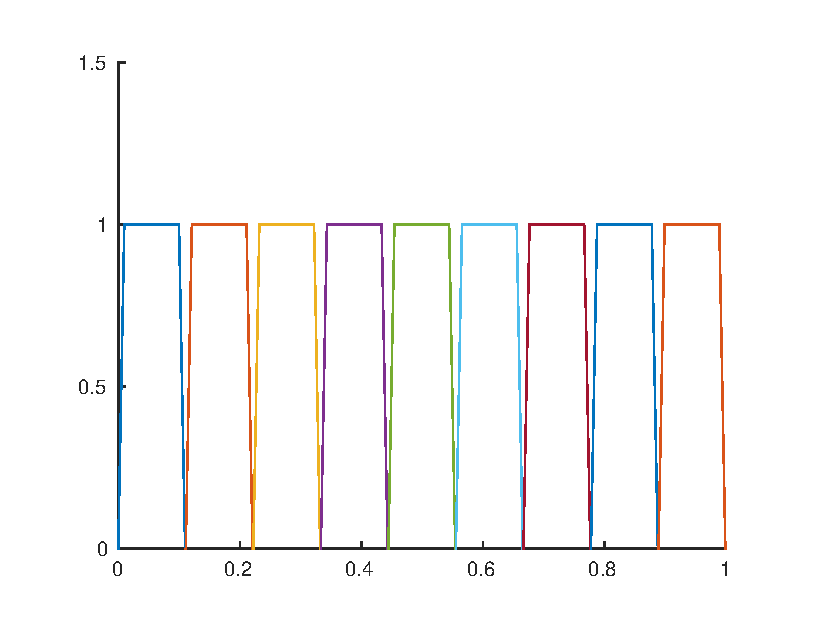
\includegraphics[width=.3\linewidth]{basis_constant.eps}}
  \label{fig:bspline_basis_constant}
\end{subfigure}%
\begin{subfigure}[B-spline basis for $p=1$]{
  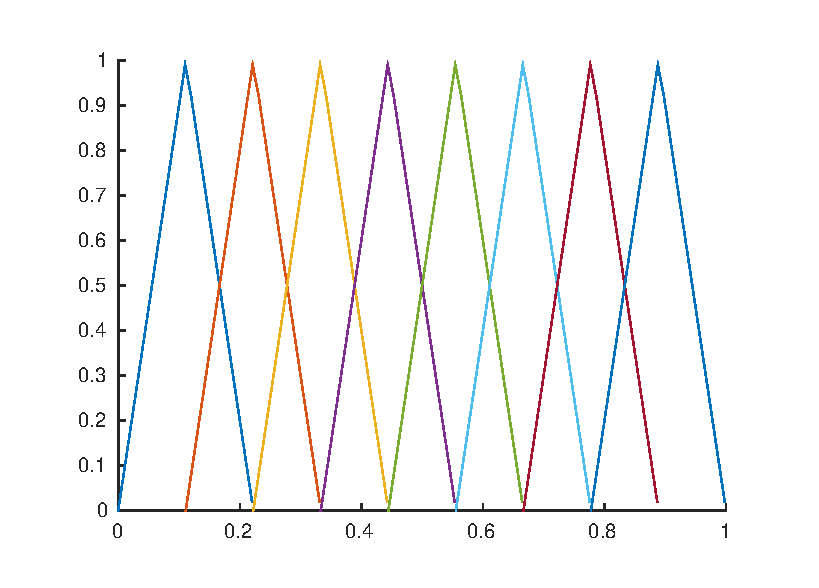
\includegraphics[width=.3\linewidth]{basis_linear.eps}}
  \label{fig:bspline_basis_linear}
\end{subfigure}
\begin{subfigure}[B-spline basis for $p=2$]{
  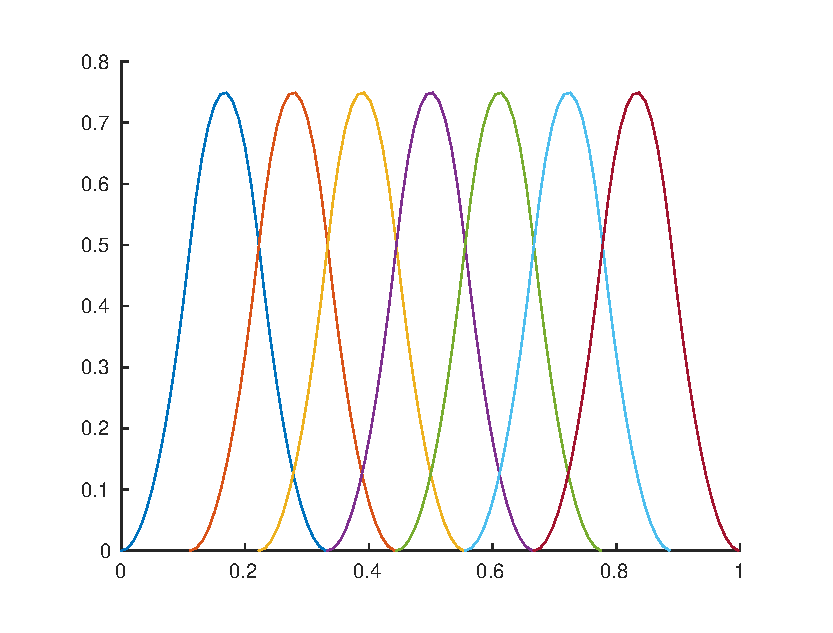
\includegraphics[width=.3\linewidth]{basis_quadratic.eps}}
  \label{fig:lognorm_quadratic}
\end{subfigure}
\caption{B-spline basis functions}
\end{figure}


Given these basis functions, Non-Uniform Rational B-Spline (NURBS) curve is given by:
\begin{equation}
C(u) = \frac{\sum_{i=1}^{k}N_{i,n}\omega_{i}P_{i}}{\sum_{i=1}^{k}N_{i,n}\omega_{i}},
\end{equation}
where $k$ is number of points, $\{P_{i}\}$ are given control points.

B--splines are have the following properties, which are useful for our problem:
\begin{itemize}
\item Degree $n$ and number of control points $\vec{P}_{i\cdots m}$ are independent.
\item B--Splines only change locally (depends on the degree $n$) when a control point is changed.
\end{itemize}

Analogically, one can define B--spline surfaces. For more information about NURBS see \cite{farin1999nurbs}.
\subsection{Minimization problem}
Now, once we defined all necessary tools, we proceed to the fitting problem.\\
The goal is to fit in a parametric curve to the set of given data points. In our case our given set of points is a mesh, obtained from surface contouring.
\subsection{Minimization Problem: Bezier curve}
First we want to find a Bezier--curve $\vec{B}_n\left(t\right)$ of degree $n$ which is approximating a given spline $\vec{s}_m\left(t\right)$ defined by $m$ points in a optimal way. For this purpose we want to minimize the L2--error. This leads to the minimization problem:
\begin{equation}
\text{find\ } \underset{\vec{B}_n\in \mathbb{B}_n}{\min} \Ltwonorm{\vec{B}_n-\vec{s}_m}
\end{equation}

Minimizing the L2--norm is equal to minimizing the functional:
\begin{equation}
F(\vec{B}_n)=\int\limits_{t=0}^{t=1} \left(\vec{B}_n-\vec{s}_m\right)^2\dt
\end{equation}

Using the variational principle we get the the system of linear equations
\begin{equation}
A a = b
\end{equation}
where $A$ is the matrix of pair-wise scalar products of basis functions (Bernstein polynomials), $b$ is the vector of scalar products of the given spline $s_{m}$ and basis functions and $a$ is a required vector of coefficients for Bezier curve representation.

\subsection{Minimization problem (least squares): NURBS}
Although the approach used above showed good results, it appears to be very computationally intensive. Analogically, one could reduce the original problem to the \textit{linear regression problem}, which allows us to reduce computational costs. Also, to improve the locality of our solution, from now on we are going to use NURBS basis functions with weights $\omega_{j} = 1$ instead of Bezier curves. For this purpose, we adopted an algorithm, provided in \cite{becker2011advanced}.

Let $X^{0}$ be the $n \times 2$ matrix of the given set of points, $N^{p}$ - the basis functions of degree $p$ ($n \times (n+p)$ matrix, where $n$ - number of points), $P^{0}$ - the control points ($(n+p) \times 2$ matrix).

The original problem can be written as:
\begin{equation}
X_{i}^{0} = \sum\limits_{j=1}^{n+p} P_{j}^{0} N_{i,j}^{p}, \quad i \in \{1,..,n\}
\end{equation}
Or, in short:
\begin{equation}
X^{0} = N^{p} P^{0}
\end{equation}
The above system needs to be solved for the unknown $P^{0}$. One of the ways to solve it is to use SVD decomposition. 
%part of implementation

\subsection{Fitting pipeline}
\begin{figure}
\centering
  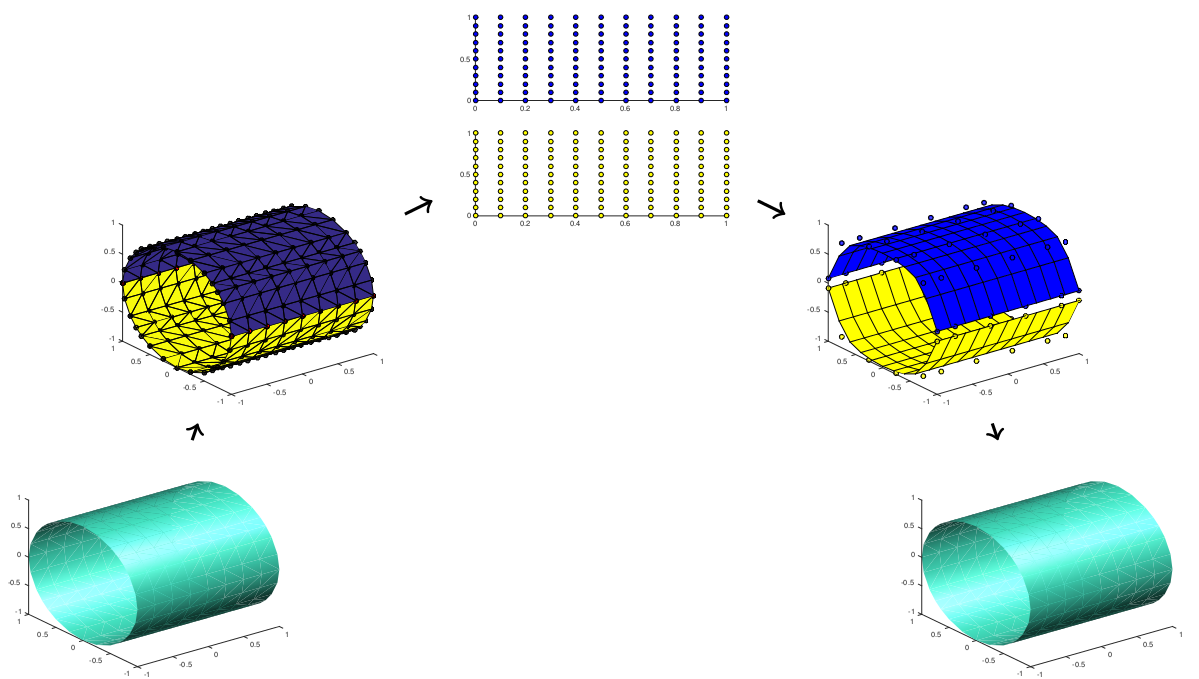
\includegraphics[width=.85\linewidth]{Fitting_workflow.png}
  \caption{NURBS fitting pipeline}
  \label{fig:fitting_pipeline}
\end{figure}
Since the geometry obtained after topology optimization can be arbitrary complex, we might not be able to find a good fit using only one patch. We seek a multi step algorithm, allowing us to break the overall big problem into smaller problems, which can be handled relatively easy.
Based on the algorithm described in \cite{eck1996automatic}, our overall fitting pipeline looks as follows (see fig. \ref{fig:fitting_pipeline}):
\begin{itemize}
	\item Patch selection (breaking our problem in small pieces which can be solved using least squares)
	\item Parametrization of obtained patches
	\item B--spline fitting using least squares
	\item Smooth connection of patches
	\item Conversion back to CAD
\end{itemize}

The pipeline given above, once implemented, will provide us with a flexible algorithm for converting an arbitrary complex mesh based geometry into NURBS and, hence, CAD--representation.
